\documentclass{resume}
\usepackage{zh_CN-Adobefonts_external, tabu, multirow, linespacing_fix, cite, titlesec, graphicx, amsmath, fontawesome5,eso-pic}

% 格式设置保持不变
\titlespacing*{\section}{0pt}{0.5ex plus 0.2ex minus 0.2ex}{0.5ex plus 0.2ex}
\titlespacing*{\subsection}{0pt}{0.5ex plus 0.2ex minus 0.2ex}{0.5ex plus 0.2ex}
\setlength{\parskip}{0.5ex}
\setlength{\itemsep}{0.5ex}

% 证件照路径已隐去
\AddToShipoutPictureBG*{%
  \AtPageLowerLeft{%
    \put(456,701){%
      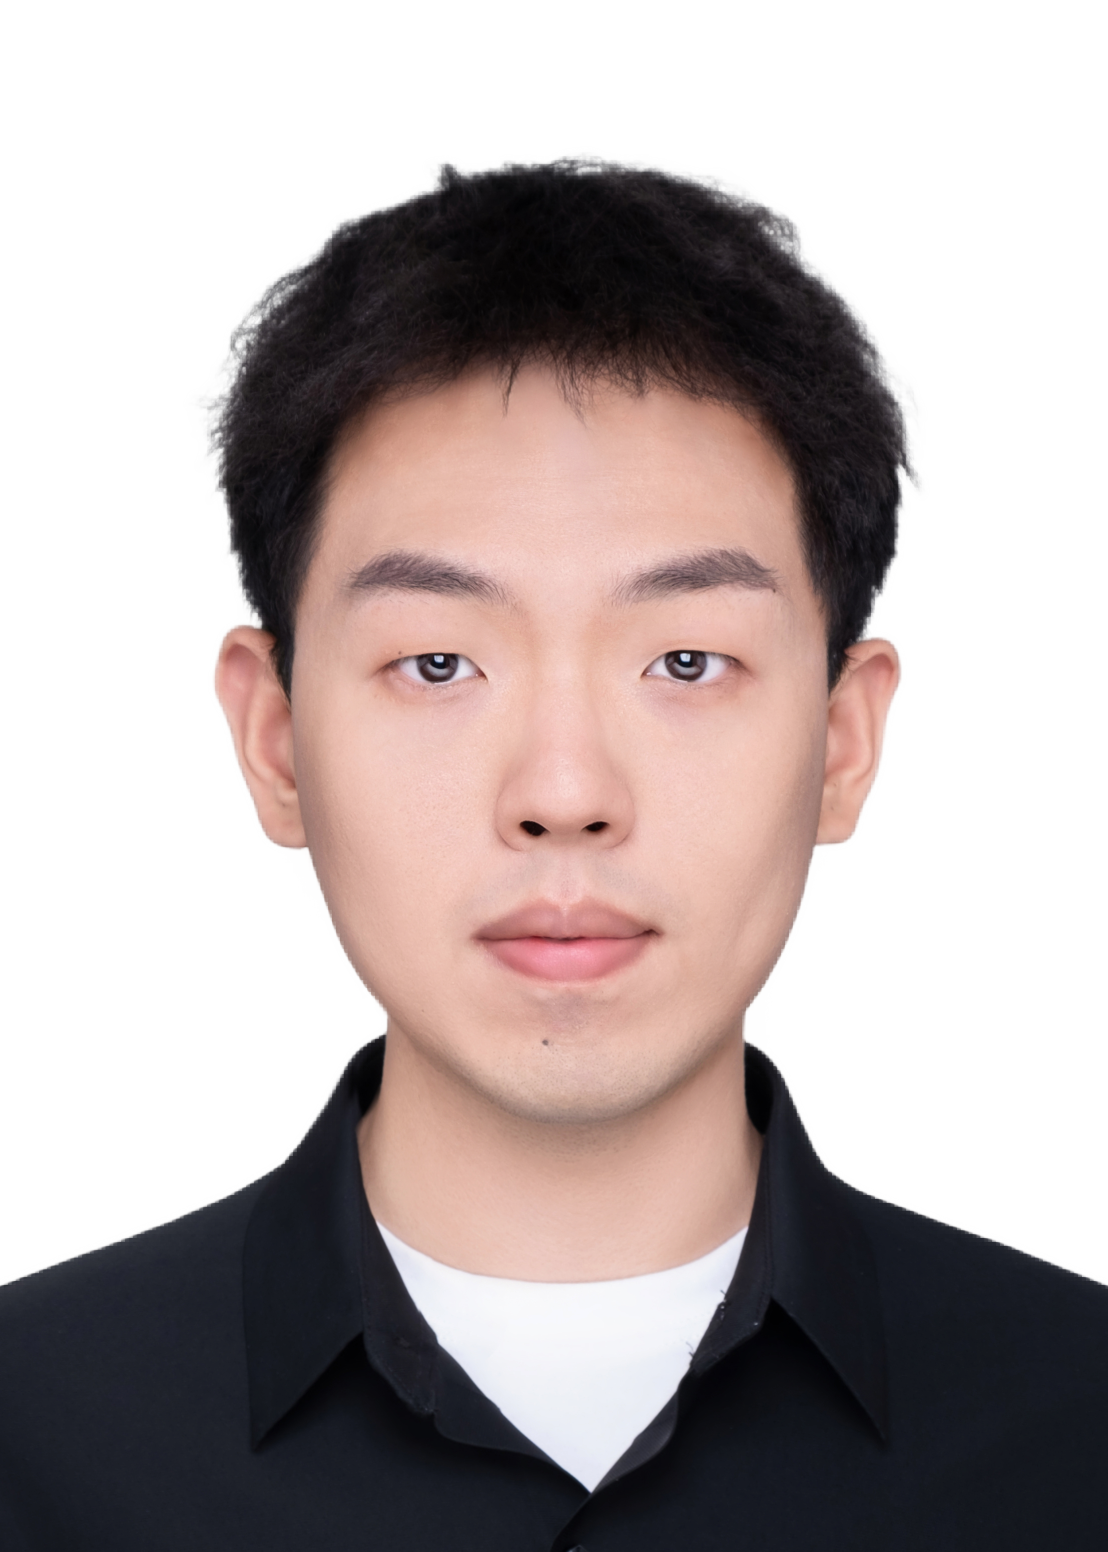
\includegraphics[width=1.15in]{avatar}
    }%
  }%
}

\begin{document}
\pagestyle{empty}

\name{[Name]}
\basicInfo{
    \email{[Email]} \textperiodcentered\ 
    \phone{[Phone]} \textperiodcentered\ 
    \text{Born in [Month] [Year]}
  }
\basicInfo{Strong language proficiency, technical expertise and teamwork capabilities}

\section{\faGraduationCap\ Education}
\datedsubsection{\textbf{Domestic University A, International University B (Top 200 QS Ranking)}}{[Start Year]-[End Year]}
\textbf{Dual Master's Degree in Computer Science and Data Science} \\
Core Courses: Data Structures, Project Management, Database Systems, Machine Learning, Cryptography, Data Mining, Network Security \\
Awarded \textbf{Full Tuition Scholarship}, Standardized Test Score: Overall [X] (Reading [X], Listening [X]) \\
Leadership Role in Student Organization, Responsible for Administrative Management, Received University-level Leadership Award

\datedsubsection{\textbf{Domestic University C}}{[Start Year]-[End Year]}
Bachelor of Engineering in Engineering Science (GPA [X]), Minor in Language Studies \\
\textbf{University Honor Roll, Merit-based Scholarship, National Academic Competition Award}

\section{\faUsers\ Work Experience}
\datedsubsection{\textbf{Financial Technology Company - Operations Engineer}}{[Start Year]-[End Year]}
\begin{itemize}
  \item Designed and implemented cloud-based disaster recovery solutions for production environments
  \item Optimized Python scripts with command-line parameterization for selective function execution
  \item Conducted hardware capacity planning and storage architecture optimization for database systems
  \item Led containerization migration project from Docker-Compose to Kubernetes for data services
\end{itemize}

\section{\faUsers\ Project Experience}
\datedsubsection{\textbf{Multimodal Physiological Monitoring System}}{[Start Year]-[End Year]}
Computer Vision, Deep Learning, Python, National-level Research Project Participation
\begin{itemize}
  \item Developed non-contact physiological signal extraction algorithm using computer vision techniques
  \item Designed hybrid CNN-LSTM architecture for multimodal feature fusion
  \item Proposed lightweight network optimization achieving 50\% reduction in computational resources
  \item Research published in SCI-indexed journal (中科院分区[X]区, IF=[X])
\end{itemize}

\datedsubsection{\textbf{Autonomous Inspection Robot System}}{[Start Year]-[End Year]}
Robotics Engineering, Path Planning, Computer Vision
\begin{itemize}
  \item Served as Project Lead responsible for technical strategy and team coordination
  \item Invented core mechanism with pending patent application
  \item Awarded Provincial-level Innovation Competition Prize
\end{itemize}

\section{\faHeartO\ Research Experience}
\datedsubsection{\textbf{Efficient Knowledge Graph Construction for Small Sample Datasets}}{[Start Year]-[End Year]}
\begin{itemize}
  \item Addressed challenge of balancing model accuracy and inference speed in named entity recognition
  \item Proposed CNN+Bi-LSTM+Attention architecture achieving state-of-the-art performance with 2x speedup
  \item Research presented at international conference (CCF Category [X] Conference)
\end{itemize}

\end{document}
